\section{Polynomial Appell mesh and uniform Lerch zero thresholds}
\label{mesh:sec:main}

The incoming uniform-continuation article asks whether the roots of the
reciprocal-gamma Appell polynomials admit a polynomial lower separation
bound. Its estimate $(3n)^{-(n-2)}$ gives an effective zero theorem, but
only a logarithmic growing-index range. We prove
\begin{equation}\label{mesh:eq:main-mesh}
 \boxed{\mesh(Q_n)\geq\frac1{10n^2}\qquad(n\geq2).}
\end{equation}
A second improvement replaces a worst-distance estimate by a harmonic
sum over the entire root configuration. Together these give a sufficient
Lerch saturation threshold of order $n^4\log^2 n$, and a relative
location error independent of $n$. The constants below are explicit
and deliberately conservative; no sharp mesh asymptotic is asserted.

\subsection{Definitions and the strengthened zero theorem}

Define the monic Appell polynomials by
\begin{equation}\label{mesh:eq:Q}
 \frac{e^{xt}}{\Gamma(1+t)}
   =\sum_{n\geq0}Q_n(x)\frac{t^n}{n!},
 \qquad W_\rho(t)=\frac1{1-\rho e^{-t}}\quad(0\leq\rho\leq1).
\end{equation}
For $n\geq0$, $k\geq1$ and $a>0$, put
\begin{equation}\label{mesh:eq:family}
 F_{n,k}^\rho(a)=\int_0^\infty
      t^k e^{-at}W_\rho(t)Q_n(\log t)\dd t.
\end{equation}
This is the manuscript's signed derivative family:
\[
 F_{n,k}^\rho=(-1)^{n+k}D_{n,k}^\rho,
 \qquad
 D_{n,k}^\rho(a)=
 \begin{cases}
  \partial_a^k\displaystyle\sum_{m\geq0}
       \dfrac{\rho^m\log^n(a+m)}{a+m},&0\leq\rho<1,\\[2mm]
  \gamma_n^{(k)}(a),&\rho=1.
 \end{cases}
\]
The endpoint $\rho=1$ unifies the derivatives, not the generally
divergent undifferentiated Lerch series. The Mellin derivation of
\eqref{mesh:eq:family} is already established in the manuscript.
We recall below the positive-transform zero bound needed to make
our localization complete.

Write the roots decreasingly as $x_{n,1}>\cdots>x_{n,n}$, set
$c_{n,j}=e^{-x_{n,j}}$, and let $H_r=\sum_{h=1}^r h^{-1}$.

\begin{theorem}[Polynomial threshold and simultaneous location]
\label{mesh:thm:saturation}
For $n\geq2$, define the explicit integer
\begin{equation}\label{mesh:eq:threshold}
 K_n=\left\lceil\bigl(16+240n^2H_{n-1}\bigr)^2\right\rceil.
\end{equation}
For every integer $k\geq K_n$ and every $\rho\in[0,1]$,
$F_{n,k}^\rho$ has exactly $n$ positive zeros, all simple.
Numbering them increasingly as $a_{n,j,k}^\rho$, one has
\begin{equation}\label{mesh:eq:location}
 \boxed{\left|\log\frac{a_{n,j,k}^\rho}{k c_{n,j}}\right|
          <\frac8{\sqrt{k}},\qquad 1\leq j\leq n.}
\end{equation}
All assertions hold simultaneously over the entire deformation interval
and over the smallest and largest zero; no compact restriction on the
slopes $c_{n,j}$ is needed.
\end{theorem}

The proof is divided into an algebraic separation theorem and a
scale-free analytic sign-transfer theorem.

\subsection{Two distinct monotonicity statements for differential factors}

For a real-rooted polynomial, its mesh is the minimum spacing of
consecutive roots counted with multiplicity. Thus a multiple root gives
mesh zero. In this subsection $\partial$ means differentiation in $x$.

\begin{lemma}[Coordinatewise motion of ordered roots]
\label{mesh:lem:motion}
For a fixed real-rooted polynomial $p$, every ordered root of
$p+c p'$, counted with multiplicity, is nonincreasing as $c>0$ increases.
Consequently each ordered root of
\[
 P(x)=\prod_{j=1}^m(1+c_j\partial)x^n
\]
is nonincreasing in each positive parameter $c_j$ separately.
\end{lemma}
\begin{proof}
Let the distinct roots of $p$ be $r_i$, with multiplicities $m_i$.
A root of multiplicity $m_i\geq2$ is inherited with multiplicity
$m_i-1$. All other roots solve
\[
 S(x):=\sum_i\frac{m_i}{x-r_i}=-\frac1c.
\]
There is one solution in each interval between consecutive distinct
roots and one to the left of all roots. Since
$S'(x)=-\sum_i m_i/(x-r_i)^2<0$, these solutions are simple, and
\begin{equation}\label{mesh:eq:root-motion}
 \frac{\dd x}{\dd c}
   =-\frac1{c^2\displaystyle\sum_i m_i/(x-r_i)^2}<0.
\end{equation}
The inherited roots remain fixed. No moving root crosses an inherited
one, because it remains in its designated complementary interval.
This proves the first assertion and real-rootedness preservation.
For the second assertion, hold all parameters except $c_j$ fixed and
apply the first to the real-rooted polynomial produced by the other
factors. The factors commute.
\end{proof}

\begin{lemma}[Riesz mesh preservation]\label{mesh:lem:riesz}
For every real-rooted polynomial $p$ and every real $c$,
\begin{equation}\label{mesh:eq:riesz}
 \mesh(p+c p')\geq\mesh(p).
\end{equation}
\end{lemma}
\begin{proof}
This classical theorem is recorded in~\cite[Theorem~1]{BKS2016}.
Here is the relevant argument. If $0<h<\mesh(p)$, then $p(x)$ and
$p(x-h)$ have interlacing roots. The real-rooted-pencil criterion says
that two real-rooted polynomials interlace if and only if every real
linear combination is real-rooted or zero. To recall why, after common
roots are removed, the partial fractions of their quotient have residues
of one sign precisely in the interlacing case. Its imaginary part then
has a fixed nonzero sign in the upper half-plane, so it takes no real
value there. Conversely, if every real pencil member has real roots,
the quotient takes no real value in that half-plane; continuity fixes
the sign of its imaginary part, and approach to each pole forces the
residues to have a common sign. This gives interlacing. Common roots
can be restored, or treated by limits.

The operator $T=1+c\partial$ preserves real-rootedness and commutes
with translation. Apply it to the interlacing pencil. Every real
combination of $Tp(x)$ and $Tp(x-h)$ remains real-rooted or zero,
so the shifted pair interlaces. For a polynomial and its translate by
$h>0$, this is equivalent to mesh at least $h$. Let $h$ increase to
$\mesh(p)$. If the original mesh is zero, the assertion follows
already from real-rootedness preservation.
\end{proof}

Lemma~\ref{mesh:lem:motion} concerns the location of each root, whereas
Lemma~\ref{mesh:lem:riesz} compares a polynomial with its image under
one operator. We do not claim that the mesh of $p+c p'$ is monotone
as a function of $c$; that stronger statement is false in general.

\subsection{A Laguerre comparison with uniform spacing}

The standard Laguerre coefficient formula, differential equation and
three-term recurrence used here are collected in DLMF
\S\S18.5, 18.8 and 18.9~\cite{DLMF}. We supply the bounds explicitly.

\begin{lemma}[An equal-factor reference polynomial]
\label{mesh:lem:laguerre}
For every $n\geq3$, the roots of
\begin{equation}\label{mesh:eq:laguerre-block}
 (1+\partial)^{3n}x^n=n!L_n^{(2n)}(-x)
\end{equation}
are negative and simple. Every adjacent gap exceeds $3$, and every
root has absolute value less than $15n/2$.
\end{lemma}
\begin{proof}
More generally, for $m\geq n$, direct coefficient comparison gives
\[
 (1+\partial)^m x^n=n!L_n^{(m-n)}(-x),\qquad
 L_n^{(\alpha)}(z)=\sum_{r=0}^n
       (-1)^r\binom{n+\alpha}{n-r}\frac{z^r}{r!}.
\]
Repeated real-root preservation removes all initial multiplicities
after $n-1$ nonzero factors. The resulting polynomial has strictly
positive coefficients when $m\geq n$, so all its real roots are
strictly negative. Equivalently the Laguerre roots are positive
and simple.

Write $y=L_n^{(\alpha)}$. Its differential equation is
\[
 xy''+(\alpha+1-x)y'+ny=0.
\]
The substitution $u=x^{(\alpha+1)/2}e^{-x/2}y$ gives
\begin{equation}\label{mesh:eq:laguerre-normal}
 u''+q(x)u=0,\qquad
 q(x)=\frac{2n+\alpha+1}{2x}
       +\frac{1-\alpha^2}{4x^2}-\frac14.
\end{equation}
For $\alpha=2n$, maximizing the quadratic in $1/x$ yields
\begin{equation}\label{mesh:eq:potential-bound}
 q(x)\leq\frac{12n^2+8n+2}{16n^2-4}\leq1\quad(n\geq3).
\end{equation}
Indeed the difference of denominator and numerator is
$4n^2-8n-6=4(n-3)^2+16(n-3)+6>0$.
If $\lambda_i<\lambda_{i+1}$ are consecutive positive Laguerre roots,
then $u$ vanishes at both endpoints of this interval. Integration by
parts and the Dirichlet Wirtinger inequality imply
\[
 \frac{\pi^2}{(\lambda_{i+1}-\lambda_i)^2}
       \int_{\lambda_i}^{\lambda_{i+1}}u^2\dd x
 \leq\int_{\lambda_i}^{\lambda_{i+1}}(u')^2\dd x
 =\int_{\lambda_i}^{\lambda_{i+1}}q u^2\dd x
 \leq\int_{\lambda_i}^{\lambda_{i+1}}u^2\dd x.
\]
Thus every gap is at least $\pi>3$.

For the largest root, the monic Laguerre recurrence identifies the
zeros with the eigenvalues of the symmetric tridiagonal matrix having
\[
 J_{ii}=2i-1+\alpha\quad(1\leq i\leq n),\qquad
 J_{i,i+1}=J_{i+1,i}=\sqrt{i(i+\alpha)}.
\]
At $\alpha=2n$, each diagonal is at most $4n-1$, and each
nonzero off-diagonal is less than $\sqrt3\,n$. The row-sum
bound for eigenvalues therefore gives
\[
 \lambda_n\leq(4+2\sqrt3)n-1<\frac{15n}{2},
\]
where $\sqrt3<7/4$. This proves both estimates.
\end{proof}

\subsection{Selecting a remote block from the gamma product}

\begin{theorem}[Polynomial reciprocal-gamma root separation]
\label{mesh:thm:polynomial}
For every integer $n\geq2$, $Q_n$ has $n$ distinct real roots and
satisfies \eqref{mesh:eq:main-mesh}.
\end{theorem}
\begin{proof}
First take $n\geq3$, and set $M=15n^2$, $m=3n$. Consider the finite
block
\begin{equation}\label{mesh:eq:remote-block}
 B_n(x)=\prod_{j=M}^{M+m-1}(1+\partial/j)x^n.
\end{equation}
Let $r_1<\cdots<r_n<0$ be the roots of the equal-factor polynomial
in \eqref{mesh:eq:laguerre-block}, and $R_1<\cdots<R_n$ those
of $B_n$. Put $c_+=1/M$ and $c_-=1/(M+m-1)$. Every coefficient
of a differential factor in \eqref{mesh:eq:remote-block} lies
between $c_-$ and $c_+$. Lemma~\ref{mesh:lem:motion}, together
with homogeneity of an equal-factor block, gives
\begin{equation}\label{mesh:eq:sandwich}
 c_+r_i\leq R_i\leq c_-r_i\qquad(1\leq i\leq n).
\end{equation}
The inequalities have this orientation because all $r_i$ are negative.
Write $R_i=c_+r_i+\eps_i$. By Lemma~\ref{mesh:lem:laguerre},
\[
 0\leq\eps_i< E,\qquad
 E=\frac{45n^2}{2M^2},
\]
since
\[
 (c_+-c_-)\frac{15n}{2}
 <\frac{m}{M^2}\frac{15n}{2}=E.
\]
The errors lie on the same side of the reference roots, so each gap
loses at most $E$, not $2E$. Consequently
\begin{equation}\label{mesh:eq:block-bound}
 R_{i+1}-R_i>\frac3M-E
 =\frac3{15n^2}-\frac{45n^2}{2(15n^2)^2}
 =\frac1{10n^2}.
\end{equation}

The Weierstrass product for the reciprocal gamma function yields the
finite-product Appell polynomials
\[
 Q_{n,N}(x)=\prod_{j=1}^N(1+\partial/j)(x+\gamma-H_N)^n.
\]
For every $N\geq M+m-1$, start with the block $B_n$, restore the
remaining factors, and translate by $\gamma-H_N$. All factors and
translations commute. Lemma~\ref{mesh:lem:riesz} shows that the
restored factors cannot decrease mesh; translations preserve it.
Thus $\mesh(Q_{n,N})>1/(10n^2)$.
The locally uniform convergence of the Weierstrass product implies
coefficientwise convergence $Q_{n,N}\to Q_n$. Ordered real roots
of monic fixed-degree polynomials vary continuously with the
coefficients, so the non-strict gap bound passes to the limit.
It proves simplicity as well as real-rootedness of $Q_n$.

Finally $Q_2(x)=(x+\gamma)^2-\zeta(2)$ has mesh
$2\sqrt{\zeta(2)}>2>1/40$, which handles the omitted index.
\end{proof}

The choice of a distant block is useful because its coefficients
$1/j$ vary little across $3n$ successive factors. It supplies separated
roots before any potentially troublesome infinite-product limit is
taken. The remaining gamma factors then preserve this separation.

\subsection{A scale-free sign-transfer estimate}

Let $Y_k$ have the gamma density
\begin{equation}\label{mesh:eq:gamma-density}
 \frac{k^{k+1}}{k!}y^k e^{-ky},\qquad y>0.
\end{equation}
Its shape is $k+1$ and rate is $k$.

\begin{lemma}[An exponential log-moment bound]
\label{mesh:lem:gamma-moment}
For positive integers $m,k$ with $k\geq16m^2$,
\begin{equation}\label{mesh:eq:gamma-moment}
 \E\bigl(e^{m|\log Y_k|}-1\bigr)
 \leq\sqrt{2(e^{4m^2/k}-1)}\leq\sqrt{2/3}<1.
\end{equation}
\end{lemma}
\begin{proof}
The square of $e^{m|\log y|}-1$ is either $(y^m-1)^2$ or
$(y^{-m}-1)^2$, hence is at most their sum. Cauchy--Schwarz bounds
the square of the left side of \eqref{mesh:eq:gamma-moment} by
\[
 \E Y_k^{2m}+\E Y_k^{-2m}-2\E Y_k^m-2\E Y_k^{-m}+2.
\]
The integer moments are
\[
 \E Y_k^r=\prod_{j=1}^r(1+j/k),\qquad
 \E Y_k^{-r}=\prod_{j=0}^{r-1}(1-j/k)^{-1}\quad(r\leq k).
\]
Both products are at least one. Since $k\geq4m$, logarithmic
bounds give
\[
 \log\E Y_k^{2m}\leq\frac{m(2m+1)}k\leq\frac{3m^2}k,
 \qquad
 \log\E Y_k^{-2m}\leq\frac2k\sum_{j=0}^{2m-1}j
                    \leq\frac{4m^2}k.
\]
The second estimate uses $-\log(1-u)\leq2u$ for $0\leq u\leq1/2$.
This proves the first claimed inequality. Finally $4m^2/k\leq1/4$
and $e^{1/4}\leq(1-1/4)^{-1}=4/3$ prove the second.
\end{proof}

\begin{proposition}[Root-distance sign transfer]
\label{mesh:prop:sign}
For real $s$ not a root of $Q_n$, set
\begin{equation}\label{mesh:eq:S}
 S_n(s)=\sum_{\ell=1}^n\frac1{|s-x_{n,\ell}|},
 \qquad m=\lceil1+S_n(s)\rceil.
\end{equation}
If $k\geq16m^2$, then simultaneously for $\rho\in[0,1]$,
\begin{equation}\label{mesh:eq:relative-sign}
 \left|
 \frac{(ke^{-s})^{k+1}F_{n,k}^\rho(ke^{-s})}
      {k!W_\rho(e^s)Q_n(s)}-1
 \right|\leq\sqrt{2/3}<1.
\end{equation}
In particular $F_{n,k}^\rho(ke^{-s})$ and $Q_n(s)$ have the same sign.
\end{proposition}
\begin{proof}
A direct substitution in \eqref{mesh:eq:family} gives the exact identity
\begin{equation}\label{mesh:eq:expectation}
 \frac{(ke^{-s})^{k+1}F_{n,k}^\rho(ke^{-s})}
      {k!W_\rho(e^s)Q_n(s)}
 =\E\left[
 \frac{W_\rho(e^sY_k)}{W_\rho(e^s)}
 \frac{Q_n(s+\log Y_k)}{Q_n(s)}\right].
\end{equation}
The logarithmic derivative of the weight satisfies
\[
 \left|\frac{\dd\log W_\rho(x)}{\dd\log x}\right|
 =\frac{x\rho}{e^x-\rho}\leq1.
\]
Indeed $e^x-\rho\geq1+x-\rho\geq\rho x$. This includes both
endpoints of the deformation interval. For
$R=W_\rho(e^{s+u})/W_\rho(e^s)$ one obtains
$R\leq e^{|u|}$ and $|R-1|\leq e^{|u|}-1$.
The product over polynomial roots gives
\[
 \left|\frac{Q_n(s+u)}{Q_n(s)}-1\right|
 \leq\prod_{\ell=1}^n\left(1+\frac{|u|}{|s-x_{n,\ell}|}\right)-1
 \leq e^{S_n(s)|u|}-1.
\]
Combining the two estimates yields
\[
 \left|R\frac{Q_n(s+u)}{Q_n(s)}-1\right|
 \leq e^{(1+S_n(s))|u|}-1\leq e^{m|u|}-1.
\]
Take expectations in \eqref{mesh:eq:expectation} and apply
Lemma~\ref{mesh:lem:gamma-moment}. These estimates also give the
needed absolute integrability. Since the normalized quantity lies
within distance less than one of $1$, it is positive.
\end{proof}

\subsection{Harmonic root distances and completeness of localization}

\begin{lemma}[Positive-transform zero bound]\label{mesh:lem:zeros}
For $n\geq0$, $k\geq1$ and $0\leq\rho\leq1$, the function
$F_{n,k}^\rho$ has at most $n$ positive zeros, counted with multiplicity.
\end{lemma}
\begin{proof}
A real kernel with $N$ sign changes has a Laplace transform with at
most $N$ positive zeros, counted with multiplicity, when its exponentially
weighted polynomial moments converge. One direct proof is induction.
At a sign-change point $t_0$, multiplication of the kernel by $t_0-t$
removes exactly that sign change. Its transform is
\[
 (\partial_a+t_0)F(a)
  =e^{-t_0a}\frac{\dd}{\dd a}\bigl(e^{t_0a}F(a)\bigr).
\]
Any finite collection of zeros of $F$ with total multiplicity $M$
forces at least $M-1$ zeros of the transformed function by Rolle's
theorem with multiplicities. The induction hypothesis gives $M\leq N$.
The fixed-sign case begins the induction, and the same induction
precludes an identically zero transform.

Here $Q_n(\log t)$ has $n$ simple sign changes, whereas
$t^kW_\rho(t)>0$. The bound
$W_\rho(t)\leq W_1(t)\leq1+t^{-1}$ ensures integrability at zero,
and $e^{-at}$ supplies it at infinity, also after any fixed number
of $a$-derivatives. The variation argument therefore applies.
\end{proof}

\begin{theorem}[Saturation from any mesh bound]
\label{mesh:thm:transfer}
Suppose $n\geq2$ and $\delta>0$ is a proved lower bound for
$\mesh(Q_n)$. If
\begin{equation}\label{mesh:eq:generic-threshold}
 \sqrt{k}\geq16+\frac{24H_{n-1}}\delta,
\end{equation}
then the full zero-count and location conclusions of
Theorem~\ref{mesh:thm:saturation} hold.
\end{theorem}
\begin{proof}
Set $\eta=8/\sqrt{k}$. Since $H_{n-1}\geq1$,
\eqref{mesh:eq:generic-threshold} implies $\eta\leq\delta/3$.
At either endpoint $s=x_{n,j}\pm\eta$, the distinguished root is
at distance $\eta$, while every other root obeys
\[
 |s-x_{n,\ell}|\geq|\ell-j|\delta-\eta
      \geq\frac23|\ell-j|\delta.
\]
Consequently
\begin{align}
 S_n(s)&\leq\frac1\eta+
       \frac3{2\delta}\bigl(H_{j-1}+H_{n-j}\bigr)\notag\\
 &\leq\frac{\sqrt{k}}8+\frac{3H_{n-1}}\delta.
 \label{mesh:eq:harmonic-distance}
\end{align}
Thus
\[
 m=\lceil1+S_n(s)\rceil
 \leq2+\frac{\sqrt{k}}8+\frac{3H_{n-1}}\delta
 \leq\frac{\sqrt{k}}4,
\]
where the last inequality is exactly
\eqref{mesh:eq:generic-threshold}. Proposition~\ref{mesh:prop:sign}
transfers the opposite polynomial signs at both endpoints to the
corresponding values of $F_{n,k}^\rho$, uniformly in $\rho$.

The $n$ intervals $[x_{n,j}-\eta,x_{n,j}+\eta]$ are disjoint,
because $2\eta\leq2\delta/3<\delta$. The decreasing coordinate
change $a=ke^{-s}$ gives $n$ disjoint positive intervals, each with
opposite endpoint signs, hence each containing a zero. By
Lemma~\ref{mesh:lem:zeros} these are all the positive zeros;
each interval contains exactly one, and every zero is simple.
The interval endpoints give \eqref{mesh:eq:location}, with a strict
inequality because the transferred endpoint signs are nonzero.
\end{proof}

\begin{proof}[Proof of Theorem~\ref{mesh:thm:saturation}]
Insert the proved value $\delta=1/(10n^2)$ from
Theorem~\ref{mesh:thm:polynomial} into
Theorem~\ref{mesh:thm:transfer}.
\end{proof}

\paragraph{Combining proved mesh bounds at small degrees.}
The incoming bound $\mesh(Q_n)\ge(3n)^{-(n-2)}$
\cite[Section 4]{IncomingUniform} and
Theorem~\ref{mesh:thm:polynomial} may both be retained. Set
\[
 \delta_n^{\mathrm{comb}}
   =\max\{(3n)^{-(n-2)},\,1/(10n^2)\},\qquad
 K_n^{\mathrm{comb}}
   =\left\lceil\left(16+
             \frac{24H_{n-1}}{\delta_n^{\mathrm{comb}}}\right)^2
     \right\rceil.
\]
Theorem~\ref{mesh:thm:transfer} applies with this bound too.
It uses the better old separation estimate at $n=2,3,4$ and the
polynomial estimate thereafter, while keeping the improved
$8/\sqrt{k}$ location error throughout. These remain sufficient
thresholds, not assertions about the first index at which the zero
count is saturated.

\begin{figure}[tbp]
 \centering
 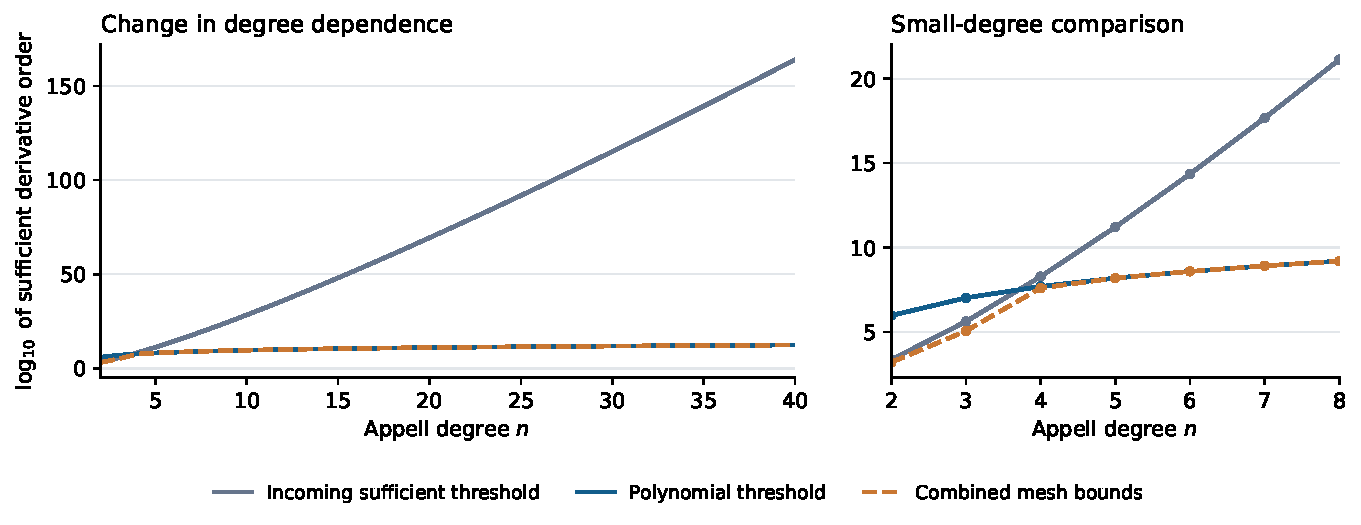
\includegraphics[width=.98\textwidth]{figures/mesh_threshold_comparison.pdf}
 \caption{Comparison of proved sufficient derivative-order thresholds.
 The incoming threshold is $576n^2(3n)^{2n-4}$.
 The polynomial threshold is \eqref{mesh:eq:threshold}, and the
 combined bound uses $\delta_n^{\mathrm{comb}}$ in the improved
 transfer theorem. The ordinate is the base-ten logarithm of each
 integer threshold; no numerical zero search is involved.}
 \label{mesh:fig:thresholds}
\end{figure}

\subsection{A polynomial growing-index regime}

\begin{corollary}[Joint growth of index and derivative order]
\label{mesh:cor:growing}
Fix $0<\alpha<1/\sqrt{60}$. For all sufficiently large integers $k$,
simultaneously for
\begin{equation}\label{mesh:eq:growing-range}
 2\leq n\leq\alpha\frac{k^{1/4}}{\sqrt{\log k}},
 \qquad 1\leq j\leq n,
 \qquad 0\leq\rho\leq1,
\end{equation}
the family has exactly $n$ simple positive zeros and satisfies
\eqref{mesh:eq:location}. In particular
\[
 \frac{a_{n,j,k}^\rho}{k e^{-x_{n,j}}}=1+O(k^{-1/2})
\]
uniformly throughout this joint range. The same conclusion holds
for any range $n=o(k^{1/4}/\sqrt{\log k})$.
\end{corollary}
\begin{proof}
The required square root of the threshold is
$16+240n^2H_{n-1}$, which increases with $n$. At the upper endpoint
of \eqref{mesh:eq:growing-range},
\[
 H_{n-1}=\bigl(\tfrac14+o(1)\bigr)\log k,
 \qquad
 \frac{16+240n^2H_{n-1}}{\sqrt{k}}
       \leq60\alpha^2+o(1)<1.
\]
The threshold condition therefore holds for all smaller $n$ too.
Theorem~\ref{mesh:thm:saturation} applies, and exponentiating its
uniform logarithmic error gives the stated relative error.
\end{proof}

\begin{remark}[Scope of the improvement]
Theorem~\ref{mesh:thm:polynomial} settles the incoming question asking
for any polynomial Appell mesh bound, with exponent $2$ and an explicit
constant. The harmonic-distance estimate also improves the transfer
argument itself. These results do not identify the actual smallest-gap
asymptotic, the sharp saturation threshold at a fixed index, or uniform
constant-offset and all-orders zero expansions when $n$ grows. The
existing fixed-index expansion remains compatible with the stronger
leading-order joint theorem proved here.
\end{remark}
